\documentclass[10pt,a4paper]{article}
\usepackage[utf8]{inputenc}
\usepackage{amsmath}
\usepackage{amsfonts}
\usepackage{amssymb}
\usepackage{multicol}
\usepackage{fullpage}
\usepackage{graphicx}
\usepackage{epstopdf}
\usepackage{tikz}
\usepackage{float}
\usepackage{booktabs}
\usepackage{listings}
\usepackage{xcolor}
\usepackage[hidelinks]{hyperref}
\usepackage{cleveref}
\usepackage[cache=false]{minted}
\usepackage{listings}

\DeclareMathOperator\erf{erf}

\definecolor{mygreen}{RGB}{28,172,0} % color values Red, Green, Blue
\definecolor{mylilas}{RGB}{170,55,241}

\author{Saran Ahluwalia and Mountain Chan}
\title{Least Squares Curve Fitting}
\begin{document}

\lstset{language=python,%
    %basicstyle=\color{red},
    breaklines=true,%
    morekeywords={matlab2tikz},
    keywordstyle=\color{blue},%
    morekeywords=[2]{1}, keywordstyle=[2]{\color{black}},
    identifierstyle=\color{black},%
    stringstyle=\color{mylilas},
    commentstyle=\color{mygreen},%
    showstringspaces=false,%without this there will be a symbol in the places where there is a space
    numbers=left,%
    numberstyle={\small \color{gray}},% size of the numbers
    numbersep=9pt, % this defines how far the numbers are from the text
    emph=[1]{for,end,break},emphstyle=[1]\color{red}, %some words to emphasise
    %emph=[2]{word1,word2}, emphstyle=[2]{style},    
}

\maketitle


\section*{Linear Least Squares}

\subsection*{Theoretical Background}

For the problem of fitting a linear least squares model to an arbitrary set of datum, $\{ (x_1, y_1), ... , (x_n, y_n)\}$ that we want to fit to an arbitrary function of the form

\begin{equation}
\sum\limits_i c_i f_i(x)
\label{eqn: arbitrary fit}
\end{equation}

An ubiquitous variant for curve fitting is to fit the data to a polynomial of order $m$. That is,

\begin{equation}
P_m(x) = \sum\limits_{k=0}^m c_k x^k
\label{eqn: general polynomial}
\end{equation}

In the following exposition, our main objective will be to fit the the error function, $\erf{(x)}$ :

\begin{equation}
\erf{(x)} = \frac{2}{\sqrt{\pi}} \int\limits_0^x e^{-t^2} dt
\label{eqn: error function}
\end{equation}

This exercise illustrates the methods for fitting a well-explored function, rather than to learn and to subsequently generalize a fitted model to an aggregated dataset.

\subsection*{Polynomial Fitting Experiments}

In this section we cover the methods for fitting a full polynomial to the $\erf{(x)}$. Briefly, the polynomial in question will possess powers for every natural number up to $n - 1$.

Plotted below are the errors of polynomial fits given by $\log \left| \erf{(x)} - P_m(x) \right|$ for a polynomial of order $m$. Plotted in this figure are polynomials with $m = 1, ..., 5$.


\begin{figure}[H]
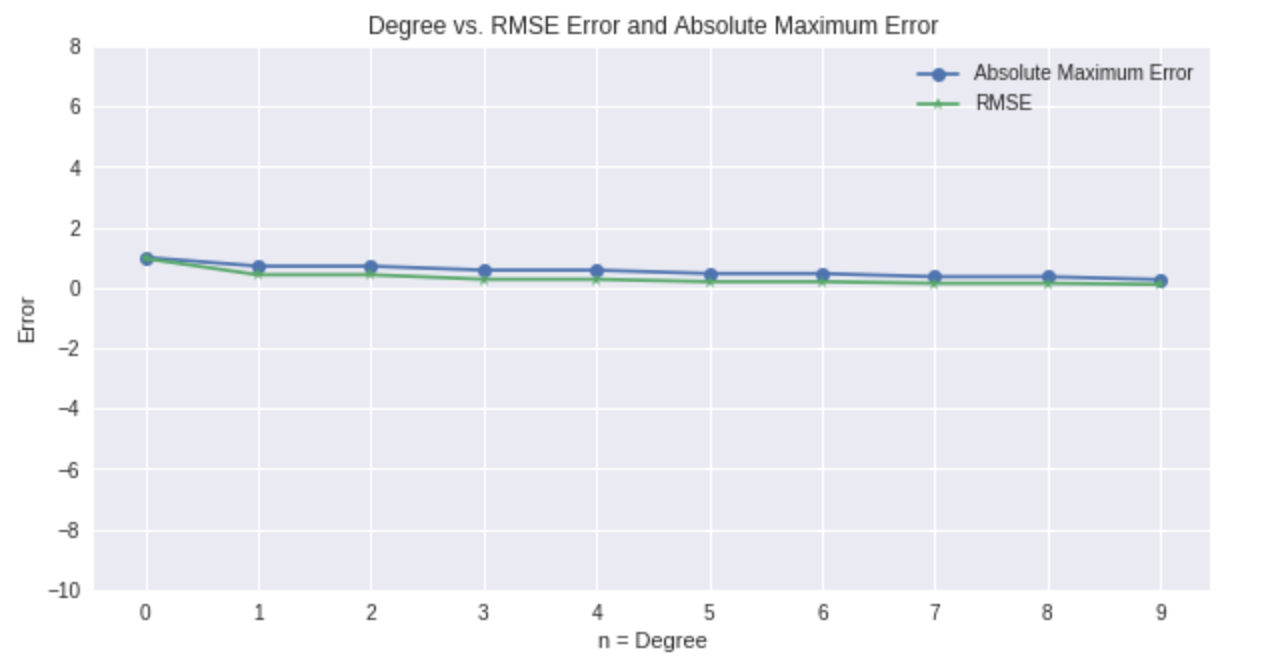
\includegraphics[scale = 0.5]{Project2/images/full_poly_error.png}
\centering
\caption{Full Polynomial Fit Error Plot}
\label{fig: fullerror}
\end{figure}

From the aforementioned data observed, \cref{fig: fullerror}, the error of each of the fit decreases as the order of the polynomial increases. This is expected as higher-order polynomials have more inflection points - hence more stability - over the image of the function, before there is an asymptotic explosion.

Note that the errors have approximate symmetry about $x=0.5$. In addition, the polynomials seem to be grouped closely into pairs of even and odd functions with a common error at $x=0.5$. Below is a table that tabulates the root mean squared error (RMSE) and the maximum absolute error (MAE) for each degree of polynomial. 

\begin{table}
\centering
\begin{tabular}{l|l|l}
Degree & Absolute Error     & RMSE                \\ \hline
0      & 0.936952448494691  & 0.9611880730344562  \\
1      & 0.35195967704345704  & 0.4243971642561228  \\
2      & 0.2169221826275908  & 0.42439716425612284 \\
3      & 0.14846721277653022  & 0.27588551185182014 \\
4      & 0.10938021110524809  & 0.27588551185182014 \\
5      & 0.07371128045209922 & 0.19567704352744125
\end{tabular}
\caption{Full Polynomial Fit Errors Values}
\label{table: fullerrors}
\end{table}

The data collected in \cref{table: fullerrors}, supports our hypothesis that the error decreased as polynomial order increased. We have included a graphical illustration of the error in \cref{fig: fullerror}. 

From this figure, we noted that the RMSE and MAE are similar. We also noted, (although we did not include the  that for $P_{10}(x)$, the RMSE and maximum errors are approximately $e^{-36} \approx 10^{-16}$. This may be due to the representation error due to how Python represents floats to IEEE-754 "double precision" standards. 754 doubles contain 53 bits of precision. Hence, during the computation of the input the computer strives to convert 0.1 to the closest fraction it can of the form $J/2^{N}$ where $J$ is an integer containing exactly 53 bits and $N$ is the number of significant digits.

\subsection*{Odd Polynomial Fitting Experiment}

Next, in order to improve the fit of the polynomial we exploited the fact that the $\erf{(x)}$ is an odd function. Hence, we decided to use odd polynomials in order to better approximate the  $\erf{(x)}$. Let the odd polynomial be represented as:

\begin{equation}
O_j(x) = \sum\limits_{k=1}^j c_k x^k
\label{eqn: odd polynomial}
\end{equation}

Where $k = 2n + 1$ for $n\in \mathbb{N}$. In this experiment, we chose $j = 1, ..., 5$ - results in polynomial degrees of 1 to 9.

Plotted below are the absolute errors of the odd polynomials. 

\begin{figure}[H]
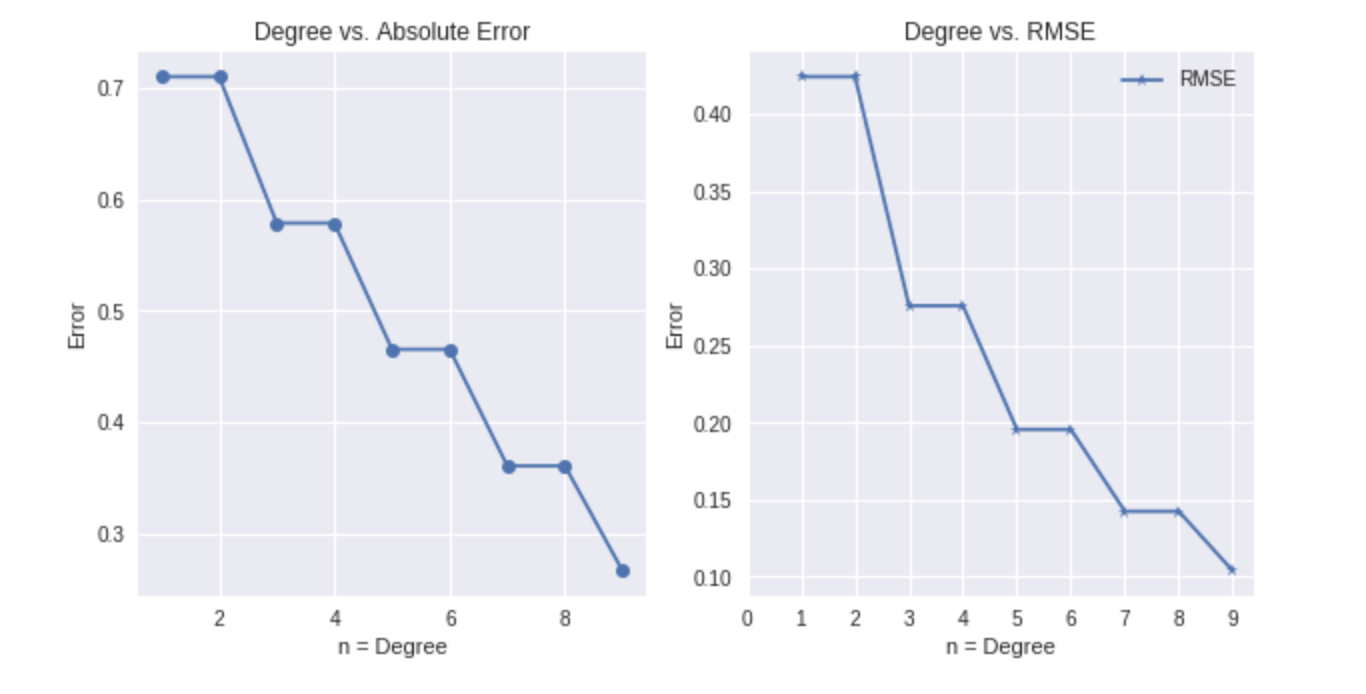
\includegraphics[scale = 0.5]{Project2/images/odd_poly_error.png}
\centering
\caption{Odd Polynomial Fit Error Plot}
\label{fig: odderror}
\end{figure}

We noted that the magnitude of the errors for the odd function were smaller than the polynomial. This is due to the fact that the pre-image of the odd function was in the interval of $x \in [-10,10]$. Had we chosen a purely non-negative pre-image, the results may be different.

\begin{table}
\centering
\begin{tabular}{l|l|l}
Degree & Absoulte Error     & RMSE                \\ \hline
1      & 0.7104739391052999 & 0.4233780400130702  \\
3      & 0.5789483075561241 & 0.2768012060313645  \\
5      & 0.46551661953661194 & 0.19821158545191792
\end{tabular}
\caption{Odd Polynomial Fit Errors Values}
\label{table: odderrors}
\end{table}

In \cref{table: odderrors}, the values of the RMSE and the MAE are listed for the odd polynomial. An intriguing trend elucidated from the corresponding polynomial of order $\frac{i+1}{2}$ was that errors were more volatile at lower degrees and more stable at higher degrees. This trend was interpreted to imply that the previous polynomial achieved numerical stability around a point. Conversely, with the odd polynomial the number of terms is halved. Hence, there will be less points that are interpolated as the function alternates between increasing and decreasing and vice versa. However, if we observe the error, we can see that although the absolute error are clearly different, the RMSE are consistent. We speculate that this may be due to the fact that the even degree for the full polynomial have coefficients that have an order of $10^{-11}$ to $10^{-16}$ whereas the coefficient for the odd degree have coefficients that have an order of $10^{-1}$ degree. The vast difference in the order of magnitude contributed little to no effects to the polynomial. Hence we have a RMSE that is very similar to each other.

Observe that even though the RMSE are closely the same, there are a huge differences in absolute error between full polynomial and odd polynomial. Thus even though the fitting are similar, absolute error tells us that full polynomial fitting is a much better fitting than the odd polynomial fitting but that is not the case when we plotted the fitting over the expected values. Hence we think that absolute error might not be a idea method for measuring error in this case, and RMSE might be a better fit for measuring and comparing error.

\subsection*{Exponential Function Fitting Experiment}

Inspection of the horizontal asymptote for the error function motivated the exploration of another means to improve the fit to the error function. The $\lim\limits_{x \to \pm \infty} \erf{(x)} = \pm1$. This poses a conundrum when applying the previous models that as it is necessary for a polynomial of order greater than zero to have the property $\left| \lim\limits_{x \to \pm \infty} P_m(x)  \right| = \infty$. 

While the exact signs can vary based on the order of polynomial and the signs of its terms, a polynomial will most certainly never have a horizontal asymptote as $x \to \pm \infty$. To fit this property of the error function, we should choose a model that has a horizontal asymptote.

One such function that possesses such a horizontal asumptope is the exponential decay function. The exponential decay function has a horizontal asymptote at $0$. At this juncture, it should be noted that this asymptote will vary depending on whether or not a constant is multiplied to the function or by simply adding as constant as another term in the model. 

The problem arises that the rest of the exponential does not have the behavior that we observe in the error function. We can absole this issue by using the product of the exponential decay and another function, which can also have a horizontal asymptote as the exponential term usually has a greater affect than other terms. The model that was chosen for this report is the following

\begin{equation}
c_1 + e^{-t^2} \left( c_2 + c_3 z + c_4 z^2 + c_5 z^3 \right)
\label{eqn: exponential model}
\end{equation}
where $z = \left( 1 + t \right)^{-1}$.

\begin{figure}[H]
\centering
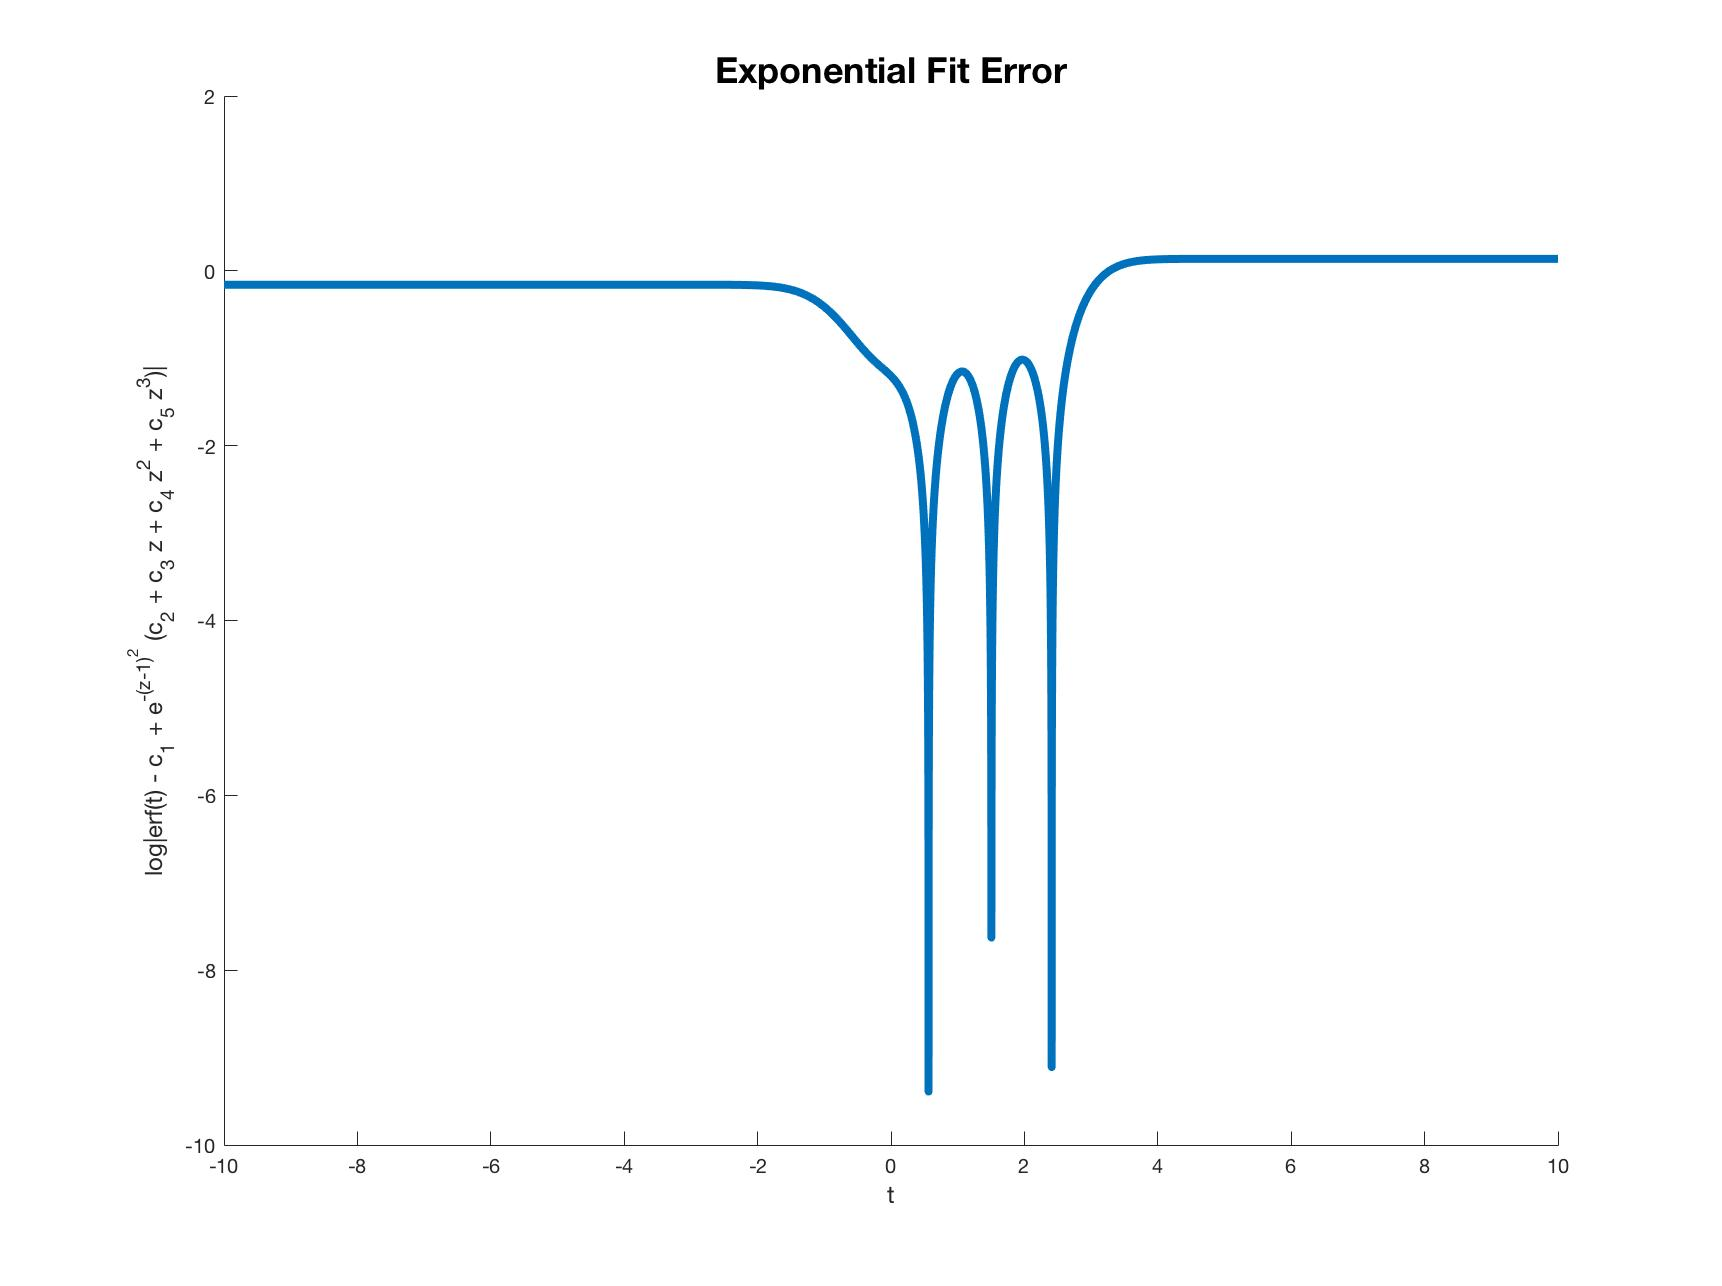
\includegraphics[scale = 0.25]{Project2/images/exp_fit_revised.jpg}
\caption{Exponential Fit Error Plot}
\label{fig: experrors}
\end{figure}

Plotted in \cref{fig: experrors} is the logarithm of the MAE of the exponential fit to the error function. This is due to the asymptotic nature of the error function and the exponential. That is, as $x$ increases, the error will decrease, with the anticipation that the error converges to zero.


Additional improvements may be made by fitting a nonlinear model, resulting in parameters in places such as exponents.


\subsection*{Python Code}

\subsubsection{Least Square Method}
\inputminted{python}{code/horner.py}

\subsubsection{Part a}
\inputminted{python}{code/full_poly.py}


\subsubsection{Part b}
\inputminted{python}{code/odd_poly.py}

\subsubsection{Part c}
\lstinputlisting[language=Matlab, caption=Exponential Model Code Sample]{code/erf_nonlinear.m}

\end{document}
